\chapter{Fourth week}

\section{Action plan}
I finished the first draft. Waiting on feedback from Dr Bhattacharya to incorporate before sending it in and inviting drs. Poortinga.

\section{Conditional Inference Trees}

% TODO: explain ctrees fully
Also called a \verb|ctree|, these are the types of decision trees that will be used to predict cancer type when given weights from the mixing matrix.

The ctree differs from normal decision trees in the way that predictor variables to split nodes on are chosen.
In a normal decision tree, one might use a metric like information gain, gain ratio, or the Gini index.
In contrast, conditional inference trees use statistical tests to determine the variable to split on as well as the split point.

To get a functional ctree in Python, the \verb|rpy2| package was used to call R code from a Python script.
The R code called to build the tree is the \verb|ctree| function from the \verb|partykit| package.
It was run with default options to understand what is happening and what output this function provides.
R's default plot method was used to visualise the tree, which involved some tweaking of label positioning.

\begin{figure}[H]
    \centering
    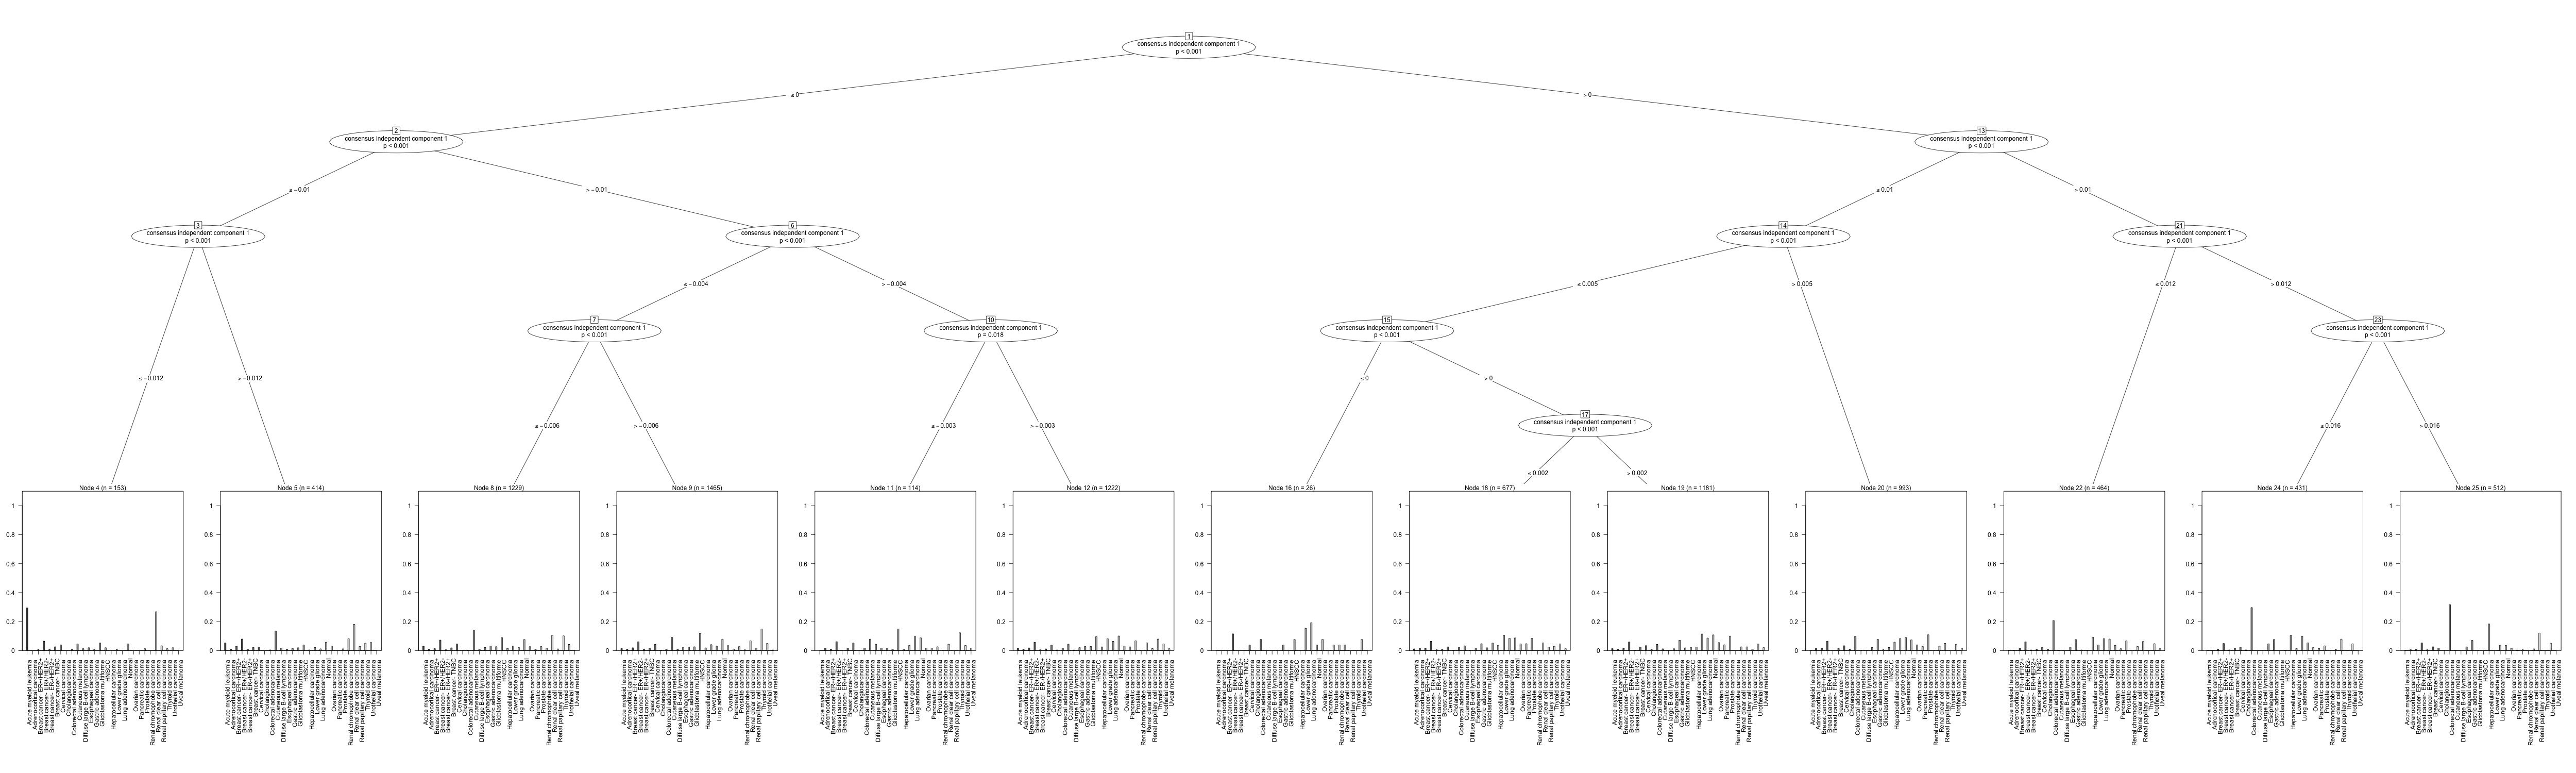
\includegraphics[scale=0.1]{ctree_default}
    \caption{A made with the partykit package, using default options}
    \label{plt:ctree_default}
\end{figure}\hspace{3cm}

\subsection{Parameters}
The \verb|ctree| function takes a few important parameters that greatly influence how the tree is built:
\begin{itemize}
    \item \verb|teststat| specifies how to choose the predictor variable to split on for a given node.
    \begin{itemize}
        \item \verb|quadratic association test| (\href{https://rdrr.io/rforge/partykitR1/f/inst/doc/ctree.pdf}{default})
        \item \verb|maximum|
    \end{itemize}
    \item \verb|splitstat| specifies how to determine the split point of the chosen predictor variable at a given node.
    \begin{itemize}
        \item \verb|quadratic association test|
        \item \verb|maximum|
    \end{itemize}
    \item \verb|splittest| a boolean value specifying whether to consider the maximum statistic value in addition to p-values.
    \item \verb|testtype| specifies the statistical test used to compute p-values.
    \begin{itemize}
        \item \verb|Teststatistic| uses the raw statistic value as criterion.
        \item \verb|Univariate| computes p-values based on the asymptotic distribution of the test statistic.
        Should be something like a t-test or equivalent.
        \item \verb|Bonferroni| works identically to \verb|Univariate| but applies Bonferroni multiple test correction.
        \item \verb|MonteCarlo| uses Monte Carlo permutation tests to assess the significance of test statistics.
        \item \verb|Univariate+MonteCarlo| combines \verb|Univariate| p-values and \verb|MonteCarlo| adjusted p-values.
    \end{itemize}
\end{itemize}

Explicitly specifying any of these options requires understanding what they mean and how they influence the tree building process.
Therefore, we'll discuss what each of these parameter options are and what they do.

\subsubsection{Quadratic association test}
